\section{Introduction}\label{sec:introduction}

% ``In this world nothing can be said to be certain, except death and taxes" \cite{sparks_jared_letter_1856}. While robots may not have to pay taxes (yet \cite{Arduengo2021}), they must battle the same force that will lead to our death and the inevitable heat death of the universe: entropy \cite{Frautschi1982}. By robots simply acting in the world around them, entropy, be it friction in their joints or an errant particle of space radiation hitting their memory, makes system failure inevitable. 
Robots are increasingly integrated into critical applications, ranging from industrial automation to healthcare and even space exploration \cite{CensusSurveyRobotic2022, Kyrarini2021, papadopoulos2021robotic}. The reliability and continuous operation of these robotic systems are crucial for their acceptance and utilization in such demanding environments. However, as robots perform tasks over extended periods, the likelihood of mechanical failures increases \cite{austin2020robotic, She2016, muirhead2012coalescing}. A particularly critical and crippling case is when multiple joints fail simultaneously. These multi-joint failures can drastically reduce the robot's task space and challenge standard motion planning algorithms due to the constraints of the robot's configuration and control spaces \cite{kingston2018sampling}.


\begin{figure}
  \centering
    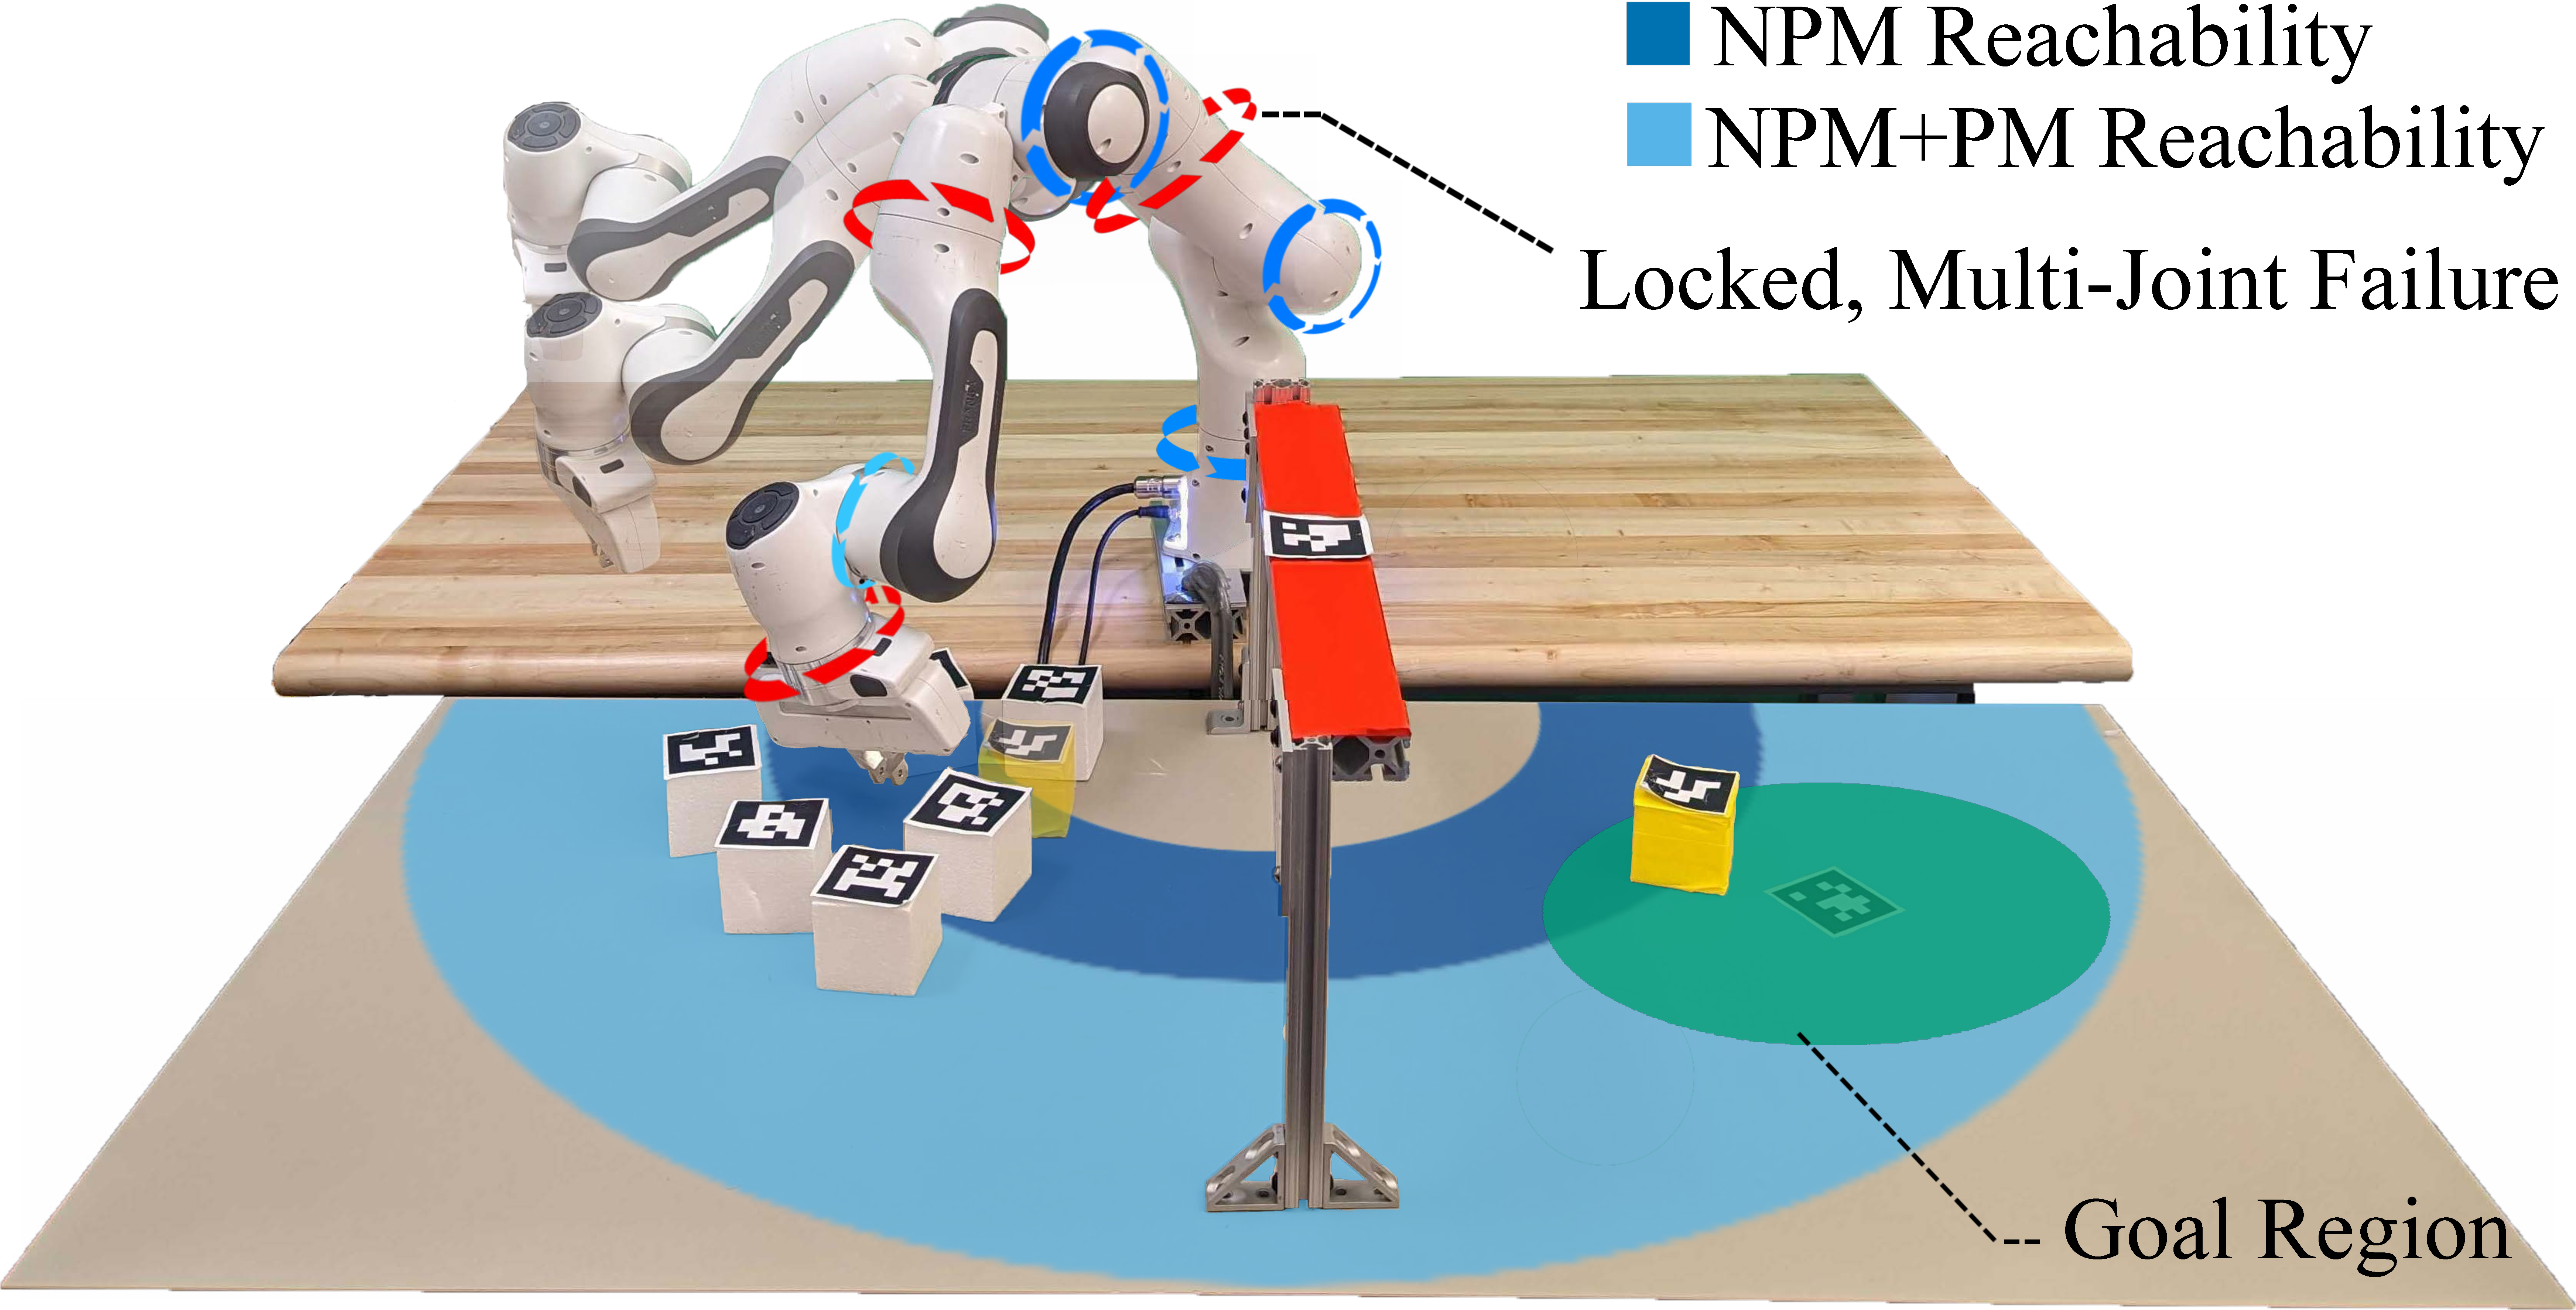
\includegraphics[width=\columnwidth]{figures/figure_1.pdf}
  \caption{This figure illustrates a robot leveraging non-prehensile manipulation (NPM) to maintain manipulation capability despite experiencing locked, multi-joint (LMJ) failures (indicated by the red rings around the joints). The robot manipulates the yellow target object from its initial position to the goal region on the right within the failure-constrained workspace represented by the blue and green regions. }\label{fig:first-page}
\end{figure}


These constraints in the robot's kinematics and dynamics can degrade its manipulation capability through reduced abilities. In this work, we define ability as a motor skill a robot can recall to manipulate an object and capability as the extent to which a robot can complete a manipulation task. For a robot manipulator that becomes underactuated due to multi-joint failures, several constraints can occur: i) the position and orientation of the end effector become coupled to the robot's remaining functional joints, ii) the manipulable area will be constrained to a subset of its non-failure size, iii) grasping may not be possible due to task constraints, such as an object being in an ungraspable orientation, iv) the robot may lose the ability to manipulate the end-effector entirely due to an adverse configuration, and v) the end effector will be subject to nonholonomic constraints \cite{Bloch_Krishnaprasad_Murray_2016}. Thus, finding a motion to connect two task-space points will require significant time to calculate or learn \cite{atreya_steering}.

To counteract the limits multi-joint failures impose on the robot's manipulation capability, we must shift the manipulation paradigm to include abilities beyond grasping and interaction beyond the end-effector. We propose using non-prehensile manipulation (NPM), or abilities corresponding to ``anything but" grasping, through contact across the whole robot embodiment, to compensate for these constraints. As seen in \cref{fig:first-page}, these new abilities will increase the robot's reachable area and enable the completion of manipulation tasks after multi-joint failure.

We adapt kinodynamic edge bundles to store NPM actions in a failure-centric map \cite{shome2021asymptotically}, a method that captures the effects of nonholonomic constraints on end effector motion. This pre-computation approach enables multi-query planning, enhancing task planning efficiency. To utilize the kinodynamic map, we developed a sim-in-the-loop task planner. By simulating actions, the planner can estimate the interactions between the robot and the environment, improving the quality of the manipulation.

This research introduces a novel method to improve manipulation capability in the event of locked, multi-joint (LMJ) failures \cite{lewis1997fault, xie2021maximizing} by using NPM abilities. The contributions of this approach are: i) modeling the failure-constrained workspace and manipulation capability of the robot, ii) generating a kinodynamic map of NPM actions across the failure-constrained workspace, and iii) a manipulation planner that uses the kinodynamic map with physical interaction simulation. We introduce a new approach to enhancing the manipulation capabilities of robots, even in the face of locked, multi-joint failures.

The remainder of this paper is structured as follows: \cref{sec:related} discusses related work, and \cref{sec:methods} describes the approach for modeling LMJs and planning under these conditions using whole-arm and NPM actions. \cref{sec:eval-design} lays out how we evaluate our approach. \cref{sec:eval} presents the experimental evaluation results, where we assess the improvements in the manipulation area and demonstrate the capability to conduct tabletop manipulation tasks under two different LMJ failure cases. \cref{sec:conclusion} concludes the paper by discussing these findings and future work.

